\documentclass[25pt,a4paper]{tikzposter}
\geometry{paperwidth=21cm,paperheight=29.7cm} % or 340 x 150 cm
\geometry{left=20mm, right=20mm, top=05mm, bottom=10mm}

%%
%\includeonly{letter2speakers}
%%

\usepackage{pdfpages} % for PDF including
%\usepackage{easyReview} % to provide a way to review (or perform an editorial process) 

\usepackage{verbatim} % to comment out
\usepackage{pgffor} % for loop
% define staff list
%\newcommand{\staffs}[1]{Abdi Fataax Jibriil Maxamed}
%\newcommand{\staffs}[1]{%
%    \ifcase#1
%    \or Tex Li-Hsing Chi
%    \or Ahmed Omer Askar
%     \fi
%}

\tikzposterlatexaffectionproofoff
\let\clearpage\relax

%\usepackage{capt-of}

% clash :-)
%\usepackage[left=20mm, right=20mm, top=30mm, bottom=20mm]{geometry}


%\usepackage{caption} % \caption*{} removal Fig. 1

%% Tikzposter is highly customizable: please see
%% https://bitbucket.org/surmann/tikzposter/downloads/styleguide.pdf
% x keeping on page one => baposter (http://www.brian-amberg.de/uni/poster/

\usepackage{multicol}
\usepackage{graphicx} % for resize table, and resize font \scalebox

% setting tikzposter; deafault {60}{72}
%\settitle{\centering{\@titlegraphic \par \bfseries \fontsize{70}{82} \sc  \@title \par}}

\usepackage{svg}
%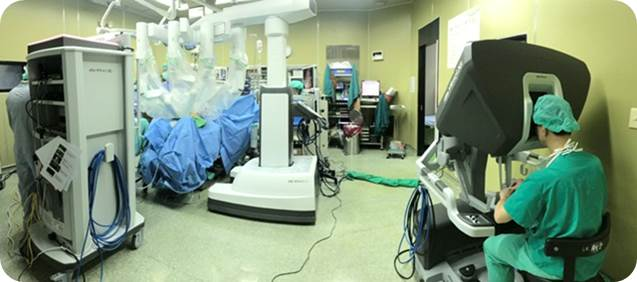
\includegraphics{TMWH_daVinci.jpg}

% a guide: https://roboticsconference.org/information/sample-poster2.pdf
% http://ctan.mirrors.hoobly.com/graphics/pgf/contrib/tikzposter/tikzposter.pdf
%% Available themes: see also
%% https://bitbucket.org/surmann/tikzposter/downloads/themes.pdf
% \usetheme{Default}
% \usetheme{Rays}
% \usetheme{Basic}
 \usetheme{Simple}
%\usetheme{Envelope}
% \usetheme{Wave}
% \usetheme{Board}
% \usetheme{Autumn}
% \usetheme{Desert}

%% Further changes to the title etc is possible
% \usetitlestyle{Default}
% \usetitlestyle{Basic}
% \usetitlestyle{Empty}
% \usetitlestyle{Filled}
% \usetitlestyle{Envelope}
% \usetitlestyle{Wave}
% \usetitlestyle{verticalShading}

\usepackage{fontspec}
\setmainfont{FreeSerif}
\setsansfont{FreeSans}
% USD500 of DFZongKaiHK-W7.otf, CrimsonText-Regular.ttf
% renamed as DFZongKaiHK.otf
\newfontfamily{\ZongKai}{DFZongKaiHK-W7.otf} %[Path=./]


\usepackage{anyfontsize}
 % Commands
 \newcommand{\bs}{\textbackslash}   % backslash
 \newcommand{\cmd}[1]{{\bf \color{red}#1}}   % highlights command
 
\newcommand{\yourName}{Dr. Tex Li-Hsing Chi, D.D.S., Ph.D.}

%    https://tex.stackexchange.com/questions/499066/how-to-increase-the-font-size-of-the-body-in-tikzposter

% https://taipeimedicaltourism.org/en/facility/detail/43

%\title{HANDOVER CEREMONY OF TRAUMA KITS FROM TAIWAN REPRESENTATIVE OFFICE FOR MINISTRY OF HEALTH DEVELOPMENT}

%{TAIWAN MEDICAL MISSION IN THE REPUBLIC OF SOMALILAND}
%\author{With electric operating tables, surgeons can easily adjust the height, lateral tilt, Trendelenburg, and reverse Trendelenburg of the table with the press of a button.}
%\institute{Taiwan Medical Mission in the Republic of Somaliland}
%% Optional title graphic

%\titlegraphic{
%\includesvg[width=0.5\linewidth]{ROC_flag.svg}
%\hspace{3cm}
%\includesvg[width=0.17\linewidth]{TMM_logo.svg}
%\hspace{3cm}
%\includesvg[width=0.5\linewidth]{Somaliland_flag.svg}
%}

% Taipei_5f994223a0add.jpg 
% https://www.mastersportal.com/search/master/medicine-health/taiwan
% 24cm
%% Uncomment to switch off tikzposter footer
% \tikzposterlatexaffectionproofoff

\begin{document}

% input or include => we use the other project instead: ASU_WelcomeRemarks_Letter
%\include{letter2speakers}
%\clearpage

\section{agenda}

%%%%%%%
%\captionsetup{labelformat=empty} % 
\begin{center} % to remove Fig.
    
\begin{tikzfigure}[]
%\begin{minipage}[b]{1\linewidth}

%Taiwan\\
%\vspace{5cm}
\includesvg[height=2.0cm, distort=false]{Flag_of_the_Republic_of_China.svg}
\hspace{2cm}
%\includesvg[width=0.17\linewidth]{TMM_logo.svg}
%\hspace{3cm}
\includesvg[height=2.0cm, distort=false]{Flag_of_Somaliland.svg}
%\captionof{Figure}{xx}
%\end{minipage}
\end{tikzfigure}

\end{center}


%%% title; font size and baseline offset (line space)
\fontsize{20}{24} \sc
2023 Collaborating for Better Health: \\
A Multi-Specialty Conference \\
%on Taiwan and Somaliland
 \par
\vspace{0.3cm}
% FOR MINISTRY OF HEALTH DEVELOPMENT

\fontsize{12}{13} \sc
Taipei Municipal Wanfang Hospital versus Hargeisa Group Hospital\\
On August 13-14, 2023, at 09:00 am, Sunday-Monday \\
Venue: Conference Hall of Carro Edeg Hotel, Hargeisa
%Exhibition Hall of the Hargeisa Group Hospital
% no more Jees Hotel
\par
%\vspace{0.2cm}
%%%%%%%%%%%%




% agenda
%\begin{columns}

%\column{0.7}
%\block{Agenda}{

\begin{center}
    
%\begin{minipage}{0.9\linewidth}

% Please add the following required packages to your document preamble:
% \usepackage{graphicx}
\begin{table}[h]
\centering
\resizebox{1.00\textwidth}{!}{%
\begin{tabular}{llll}
%%%% day 1
\textbf{August 13} & \textbf{Topic}       & \textbf{Speaker}                                                                            & \textbf{} \\ \hline  \hline

09:00         & Opening                 & \begin{tabular}[c]{@{}l@{}} \textbf{Dr. Ming-Che Lee, M.D., Ph.D.}\\ (Deputy Superintendent, TMWH)\end{tabular}    
&           \\ \hline

09:05         & History of Hemodialysis in Somaliland                 & \begin{tabular}[c]{@{}l@{}} \textbf{Dr. Ahmed Wali, M.D.}\\ (Director, Hemodialysis Center of HGH)\end{tabular}    
&           \\

%09:20         & Viral Hepatitis and Liver Disease in Somaliland                 & \begin{tabular}[c]{@{}l@{}} \textbf{Dr. Deq Said Jama, M.D.}\\ (Director, WHO Office in Hargeisa)\end{tabular}    
%&           \\

09:20         & Organ Transplantation in Wan Fan Hospital                 & \begin{tabular}[c]{@{}l@{}} \textbf{Dr. Ming-Che Lee, M.D., Ph.D.}\\ (Deputy Superintendent, TMWH)\end{tabular}    
&           \\

% MoU of Hemodialysis Center---Transplant Team
09:35         & Panel Discussion           & \begin{tabular}[c]{@{}l@{}} \textbf{Dr. Ahmed and Dr. Ming-Che}\\ 
\end{tabular}    
&           \\ \hline


10:00         & Treatment of Acute Ischemic Stroke in Taiwan                 & \begin{tabular}[c]{@{}l@{}} \textbf{Dr. Chin-I Chen, MD.}\\ (Director, Stroke Center, TMWH)\end{tabular}    
&           \\


\hline



%%%

% Hersi Dahir Madar
% Omar Marshal: How is cancer in somaliland and how is the understanding of local people and what setting is ready for them....
10:15         & Incidence and Distribution of Cancer in Somaliland   
& \begin{tabular}[c]{@{}l@{}} \textbf{Dr. Omar Marshal, M.D.} \\(Pathologist, HGH) \end{tabular}                                                &           \\ \hline

10:30         & Common Thyroid Disorders in Somaliland   & \begin{tabular}[c]{@{}l@{}} \textbf{Dr. Adnan Sayid Abdo, M.D.} \\(Deputy Director, Hargeisa Group Hospital, HGH) \end{tabular}                                                &           \\

10:45         & Common Diseases in Otolaryngology (ENT) and WFH ENT Training Program   & \begin{tabular}[c]{@{}l@{}} \textbf{Dr. Shih-Han Hung, M.D., Ph.D.} \\(Director, Department of Otolaryngology of TMWH) \end{tabular}                                                &           \\
%%%

11:00         & Maxillofacial Care for Gunshot Patients in Somaliland  & \begin{tabular}[c]{@{}l@{}} \textbf{Dr. Abdirahim Uurcade, BDS (Pak), FCPS (Pak), FAOCMF (Germany)} \\(Consultant Oral and Maxillofacial Surgeon, HGH) \end{tabular}                                                          &           \\


11:15         & The Current State of Neurosurgery in Somaliland & \begin{tabular}[c]{@{}l@{}} \textbf{Dr. Abdulhamid Mohamed Ali Suleman, M.D.} \\(Consultant Neurosurgeon, HGH) \end{tabular}                                                          &           \\

% Khat-leaf Use
%11:15         & Research Project: Fluorosis and Oral Health in Somaliland & \begin{tabular}[c]{@{}l@{}} \textbf{Dr. Tex Li-Hsing Chi, D.D.S., Ph.D.} \\(Chief, Taiwan Medical Mission) \end{tabular}              %                                            &           \\



11:30         & Panel Discussion  & \begin{tabular}[c]{@{}l@{}} \textbf{Dr. Shih-Han, Dr. Adnan, Dr. Abdulhamid, Dr. Omar, Dr. Tex, and Dr. Abdirahim}\\ (Head and Neck Surgeons) \end{tabular} &           \\  \hline

%11:20         & Emergency Ultrasound  & \begin{tabular}[c]{@{}l@{}} \textbf{Dr. Yun-yu Wu, M.D.} \\ 
%(Department of Emergency, TMWH)  \end{tabular}                                                                                     &           \\

%10:20         & Remark for the Project  & \begin{tabular}[c]{@{}l@{}} \textbf{ Mr. Allen Lou }\\ (Ambassador of Taiwan in Somaliland)\end{tabular}  &           \\

12:00         & Group Photos/Lunch Break            &                                                                                             &           \\
%12:35         & Refreshment &                                                                                             &   \\ 


%%%%%%%%%%%%%%%%%%%%%%%%% day 2
\\
\textbf{August 14} & \textbf{Topic}       & \textbf{Speaker}                                                                            & \textbf{} \\  \hline  \hline

09:00         & VIP Remarks                 & \begin{tabular}[c]{@{}l@{}} \textbf{Dr. Mohamed Abdi Hergeye, M.D.}\\ (Director General, MoHD)\end{tabular} &           \\  

09:10         & VIP Remarks  & \begin{tabular}[c]{@{}l@{}} \textbf{Amb. Allen Lou }\\ (Ambassador of Taiwan to Somaliland)\end{tabular}  &           \\ \hline

09:20         & Forensic Medicine in Somaliland   & \begin{tabular}[c]{@{}l@{}} \textbf{Dr. Ahmed Omar Askar, M.D.} \\(Director, HGH) \end{tabular}                                                &           \\

%09:20         & Forensic Medicine in Taiwan   & \begin{tabular}[c]{@{}l@{}} \textbf{Dr. Tex Li-Hsing Chi, D.D.S., Ph.D.} \\(Chief, Taiwan Medical Mission)  \end{tabular}                                                &           \\
%%% Taiwan Medical Mission,對於HGH的幫助等效益

09:35         & Panel Discussion  & \begin{tabular}[c]{@{}l@{}} \textbf{Dr. Askar and Dr. Tex}\\ (Medical Investigators) \end{tabular} &           \\  \hline

%%% 台灣捐贈的骨科設備,對於索國骨科醫師的幫助等效益
10:00         & Orthopedic Care for Gunshot Patients in Somaliland   & \begin{tabular}[c]{@{}l@{}} \textbf{Dr. Ahmed Saed Ali, M.D.} \\(Chief, Orthopedic Department of HGH) \end{tabular}                                                          &           \\

10:15         & Management of Trauma Patient in Taiwan Emergency Department  & \begin{tabular}[c]{@{}l@{}} \textbf{Dr. Yun-yu (Cloud) Wu, M.D.} \\ 
(Specialist, Emergency Department of TMWH)  \end{tabular}                                                                                     &           \\
10:30         & Panel Discussion  & \begin{tabular}[c]{@{}l@{}} \textbf{Dr. Ahmed and Dr. Yun-yu}\\ (Trauma Team) \end{tabular} &           \\  \hline

%%
11:00         & Tackling Non-communicable Diseases in Somaliland  &  \begin{tabular}[c]{@{}l@{}} \textbf{Dr. Abdirahman Madar
M.D., MSc.} \\ (Board President, Somalilander-American Health Association) \end{tabular}  &           \\ \hline

%11:20         & Introduction of Viral Hepatitis in Somaliland  &  \begin{tabular}[c]{@{}l@{}} \textbf{Dr. Abdulkani Yusuf, M.D.} \\ (Director of City Hospital) \end{tabular}                                                                                &           \\
%10:20         & Remark for the Project  & \begin{tabular}[c]{@{}l@{}} \textbf{ Mr. Allen Lou }\\ (Ambassador of Taiwan in Somaliland)\end{tabular}  &           \\

% Dr. Jinaw Mohamed Qalib, M.D., MsHPE, MPH (Clinical-Teaching Coordinator, University of Hargiesa)
11:15         & Medical Education and Internship Training in Somaliland  &  \begin{tabular}[c]{@{}l@{}} \textbf{Dr. Jinaw Mohamed Qalib, M.D., MsHPE, MPH} \\ (Clinical-Teaching Coordinator, University of Hargeisa) \end{tabular}  &           \\ \hline

11:30         & %MoU: TMM, and College of Medicine and Health Science of UoH  
&                                                                                             &           \\ %\hline
12:00         & Closure/Group Photos/Lunch Break &                                                                                             &   \\  


\end{tabular}%
} % end of resizebox


\end{table}


%\end{minipage}

\end{center}



%%%%%%%%%%%

%%% footer
%\block{}{
%\node [above right,
%       outer sep=0pt,
%       minimum width=\paperwidth-2*\pgflinewidth,
%       minimum height=7cm,
%       align=center,font=\Huge,
%       draw,fill=green!30,
%       ultra thick] at ([shift={(0.5*\pgflinewidth,0.5*\pgflinewidth)}]bottomleft) 
%       {

\begin{tikzfigure}[]
%\includesvg[height=40.0cm, distort=false]{ortho_ward_Tex_Josh.svg}

%\includesvg[height=2.5cm, distort=false]{TRO_Somaliland.svg} \hspace{2cm}
%\includesvg[height=2.5cm, distort=false]{MoHD_Somaliland.svg}

%\hspace{1cm} % https://mohd.govsomaliland.org/
%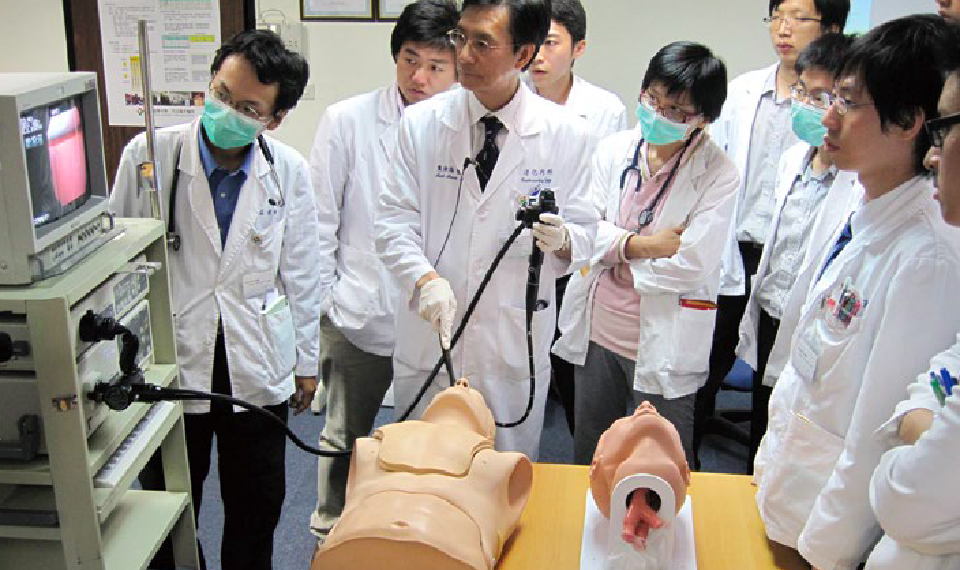
\includegraphics{TMWH_scope.pdf}


%*** using zong Kai Chinese font by \ZongKai{}, and adjust image size \scalebox{h}[v]{}
% image and character: \resizebox{2.7cm}{1.5cm}{}
\ZongKai{\fontsize{3.3}{6}\selectfont \scalebox{1.3}[1.0]{\includesvg[height=1.5cm, distort=false]{TRO_Somaliland.svg}}}
\includesvg[height=1.5cm]{TMWH_logo_TAIPEI_vector.svg}
%\includesvg[height=25.0cm, distort=false]{TRO_Somaliland_font_ZongKai.svg.svg}\hspace{1cm} % TRO logo with ZongKai font in path
\includesvg[height=1.5cm, distort=false]{TMM_logo.svg}
%{2023TMM_officePlate_pink.svg}
%\includesvg[height=1.5cm, distort=false]{Hargeisa_Group_Hospital_logo.svg}
%\includesvg[height=1.5cm, distort=false]{MoHD_Somaliland.svg} % 2020
\includesvg[height=1.5cm, distort=false]{logo_MoHD_HGH.svg} 
%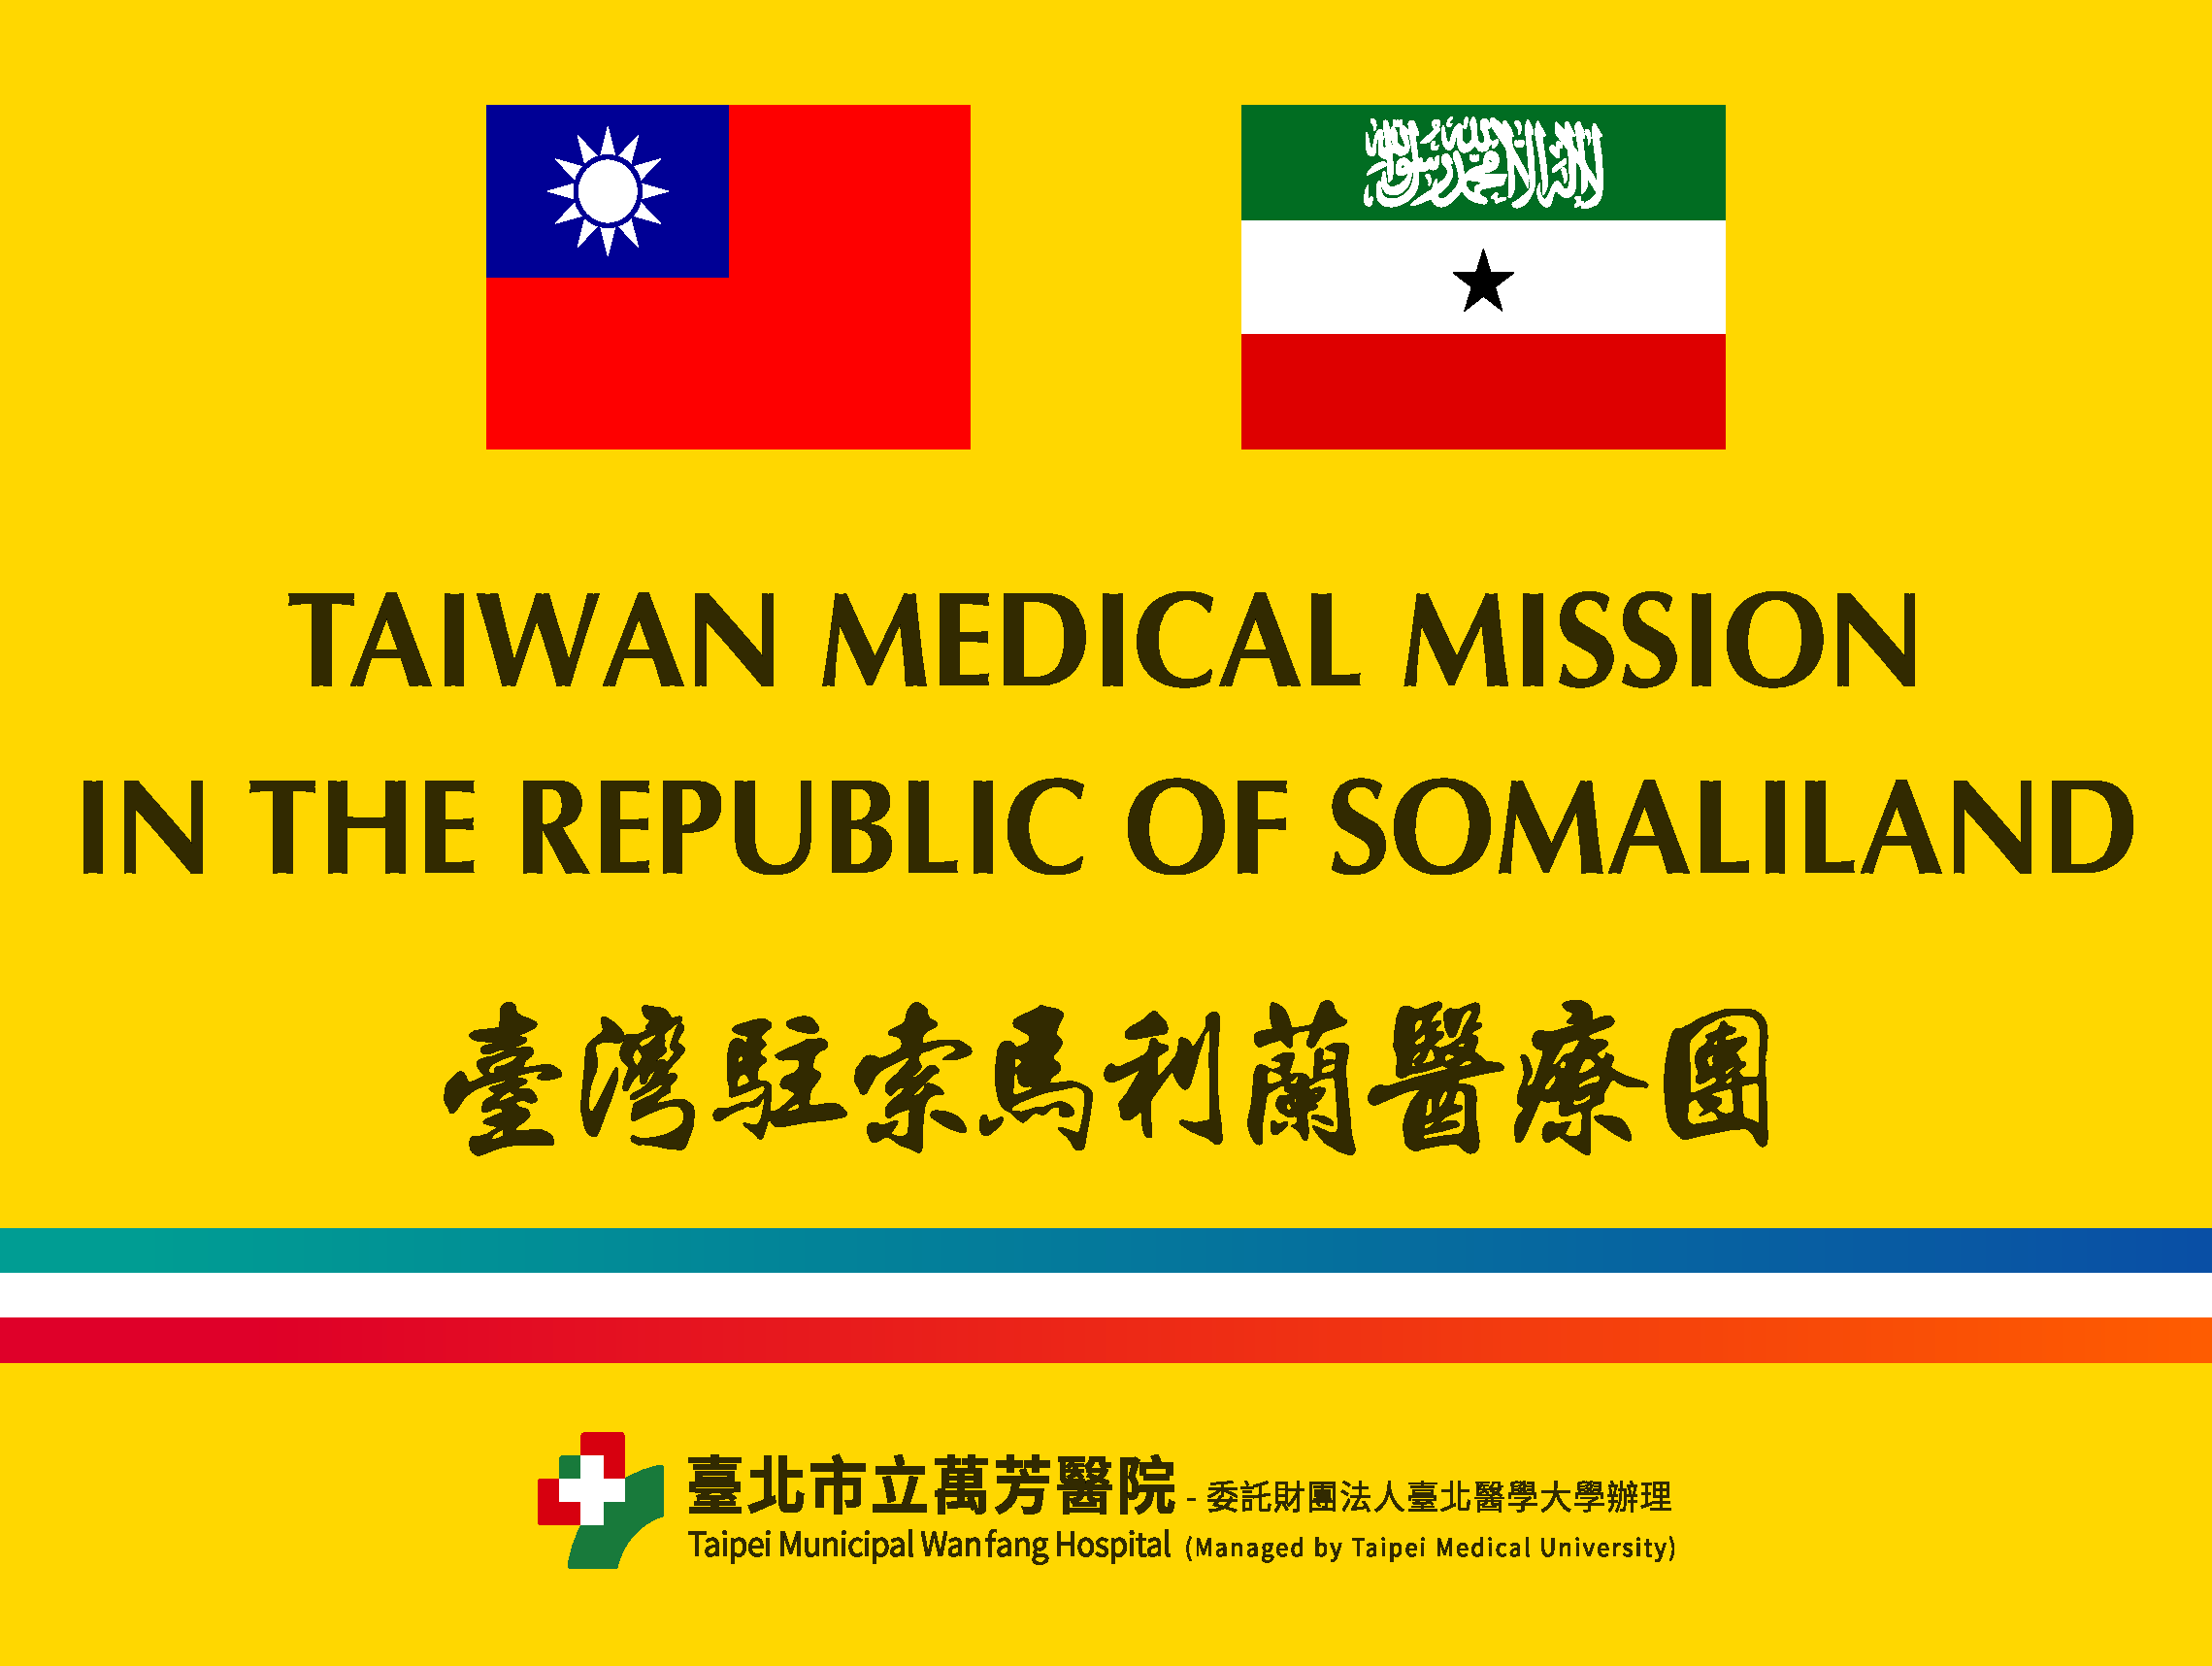
\includegraphics[height=12.0cm, distort=false]{2023TMM_officePlate_ai.pdf}

%%% *********
% ?? add logo of military and social welfare ??

\end{tikzfigure}



%}; % end of node

%} % end of block

%\clearpage


% include PDF is better
%%\documentclass{letter}
\usepackage[top=0.5in, bottom=1in, right = 1in, left = 1in]{geometry}
\usepackage{hyperref}
\usepackage{graphicx}
\usepackage{wrapfig}
\usepackage{svg, outlines}

\usepackage{lipsum}

\address{\large \textbf{Taiwan Medical Mission (TMM) } \\
\vspace{3pt} 
\large \textbf{in the Republic of Somaliland} \\
%\large \textbf{Space Exploration} 
\vspace{3pt} 
Hargeisa, Somaliland}
\date{}

\begin{document}
\begin{letter}
{
\centering \Large \textbf{Letter of Welcome Remarks}
}

\hfill
\begin{wrapfigure}[1]{l}{0.35\linewidth}%{height=0.65\textheight}
    \centering
    \includesvg[width=0.20\textwidth]{TMM_logo.svg}
\end{wrapfigure}

\opening{Dear Dr. Yun-Yu Wu,} % admissions officer
\medskip 

%\lipsum[1-5]

Subject: A brief summary of TMM, and a project of capacity building in emergency care\\
 \today



%I'm writing to you as the chief doctor who lives in your Hargeisa dormitory house with other TMM members. We appreciate your kindness and cooperation very much.

%%


I sincerely hope you are doing well as I write this email. I'm writing to welcome you to the Taiwan Medical Mission (TMM) in the Republic of Somaliland. 
We look forward to working with you.

As you may know, TMM is an oversea mission that provides healthcare for the people of Somaliland. Dr. Dave Lin, an obstetrician, Josh Huang, a registered nurse, and Dr. Tex Li-Hsing Chi, an oral and maxillofacial surgeon, make up our team of medical professionals. We work at Somaliland's Hargeisa Group Hospital (HGH) to provide service while building capacity.

Josh teaches nurses how to think critically, which enhances nursing care. We also contribute to the system and equipment upgrades in the orthopedic ward for women. 
Since June 2023, TMM's new project has included a pap smear project to screen for cervical cancer with an obstetrics and gynecology (OBS/GYN) director named Dr. Fatima and Dr. Dave's support, as well as a telepathology project with a pathologist named Dr. Omar to interpret the cytology diagnosis of a pap smear.

TMM also supports the Vitek 2 Compact bacterial identification machine, orthopedic instruments, and implants, the arthroscopic Skryker shaver, trauma kits for soldiers serving on the front lines of battle, oxygen concentrators, autoclaves, a video intubation system, and other medical devices or medicines for use in hospitals.

We work on non-communicable diseases together with non-governmental organizations (NGOs) and instruct interns at the University of Hargeisa. 
TMM does telemedicine by collaborating with specialists at Taipei Municipal Wanfang Hospital (TMWH), where TMM is based.


Additionally, we want to promote good oral hygiene and screen khat leaf chewers for oral cancer. 
The HGH medical personnel will also have access to screenings, vaccinations, and treatment options for HBV/HCV viral hepatitis program. 
%After Dr. Dave finishes his mission, an emergency doctor, Dr. Wu from TMWH will join us in July 20231.

With the help of Australian Doctors for Africa (ADFA, URL: https://ausdocafrica.org/), a project that will boost emergency care in HGH is currently underway. This initiative will train local physicians and increase the medical staff's professional expertise, enabling them to provide more systematic and thorough care. In addition, point-of-care ultrasound was implemented in the emergency department and intensive care unit (ICU) on April 2023 by Dr. Max Fraden (Somalilander-American Health Association, SAHA, urlhttps://sahainfo.org/our-vision/).
The creation of a trauma team will allow rapid responses to emergencies delivering prompt and efficient care to patients in severe conditions.

We think that constant support is essential to the accomplishment of our programs. As a result, all of our TMM members have access to mentorship, training, resources, and support networks provided by TMWH headquarters. 
We would also want to provide you with this support.

\newpage

\begin{outline}
    
Our core value is:
\1 TMM offers medical professionals for people in need.
\1 TMM's presence is supposed to bring happiness and safety to everyone around them by improving their health and well-being.
\1 When confronted with a challenge, TMM is resilient in persuading its core value.

\end{outline}

%%
I'm writing to ask if it's possible to schedule a teleconference with emergency medical personnel at Hargeisa Group Hospital. 
In order to help us to construct a comprehensive project, we think a teleconference would be beneficial prior to your arrival. The difficulty of delivering medical supplies to Somaliland should have prompted us to start working on this earlier.


We appreciate your thoughts and time. We hope to hear from you shortly. You can contact me at any time via email or WhatsApp (we create a group for you: HGH-ED Taiwan Medical Mission).

%I appreciate your time. If you have any questions or issues about our plan, kindly let us know. 




\medskip
Regards, \\ \\ \\
Dr. Tex Li-Hsing Chi, D.D.S., Ph.D.\\
Chief, \\
Taiwan Medical Mission\\
texchi2@gmail.com\\
+252(0)637772613


\end{letter}
\end{document}
%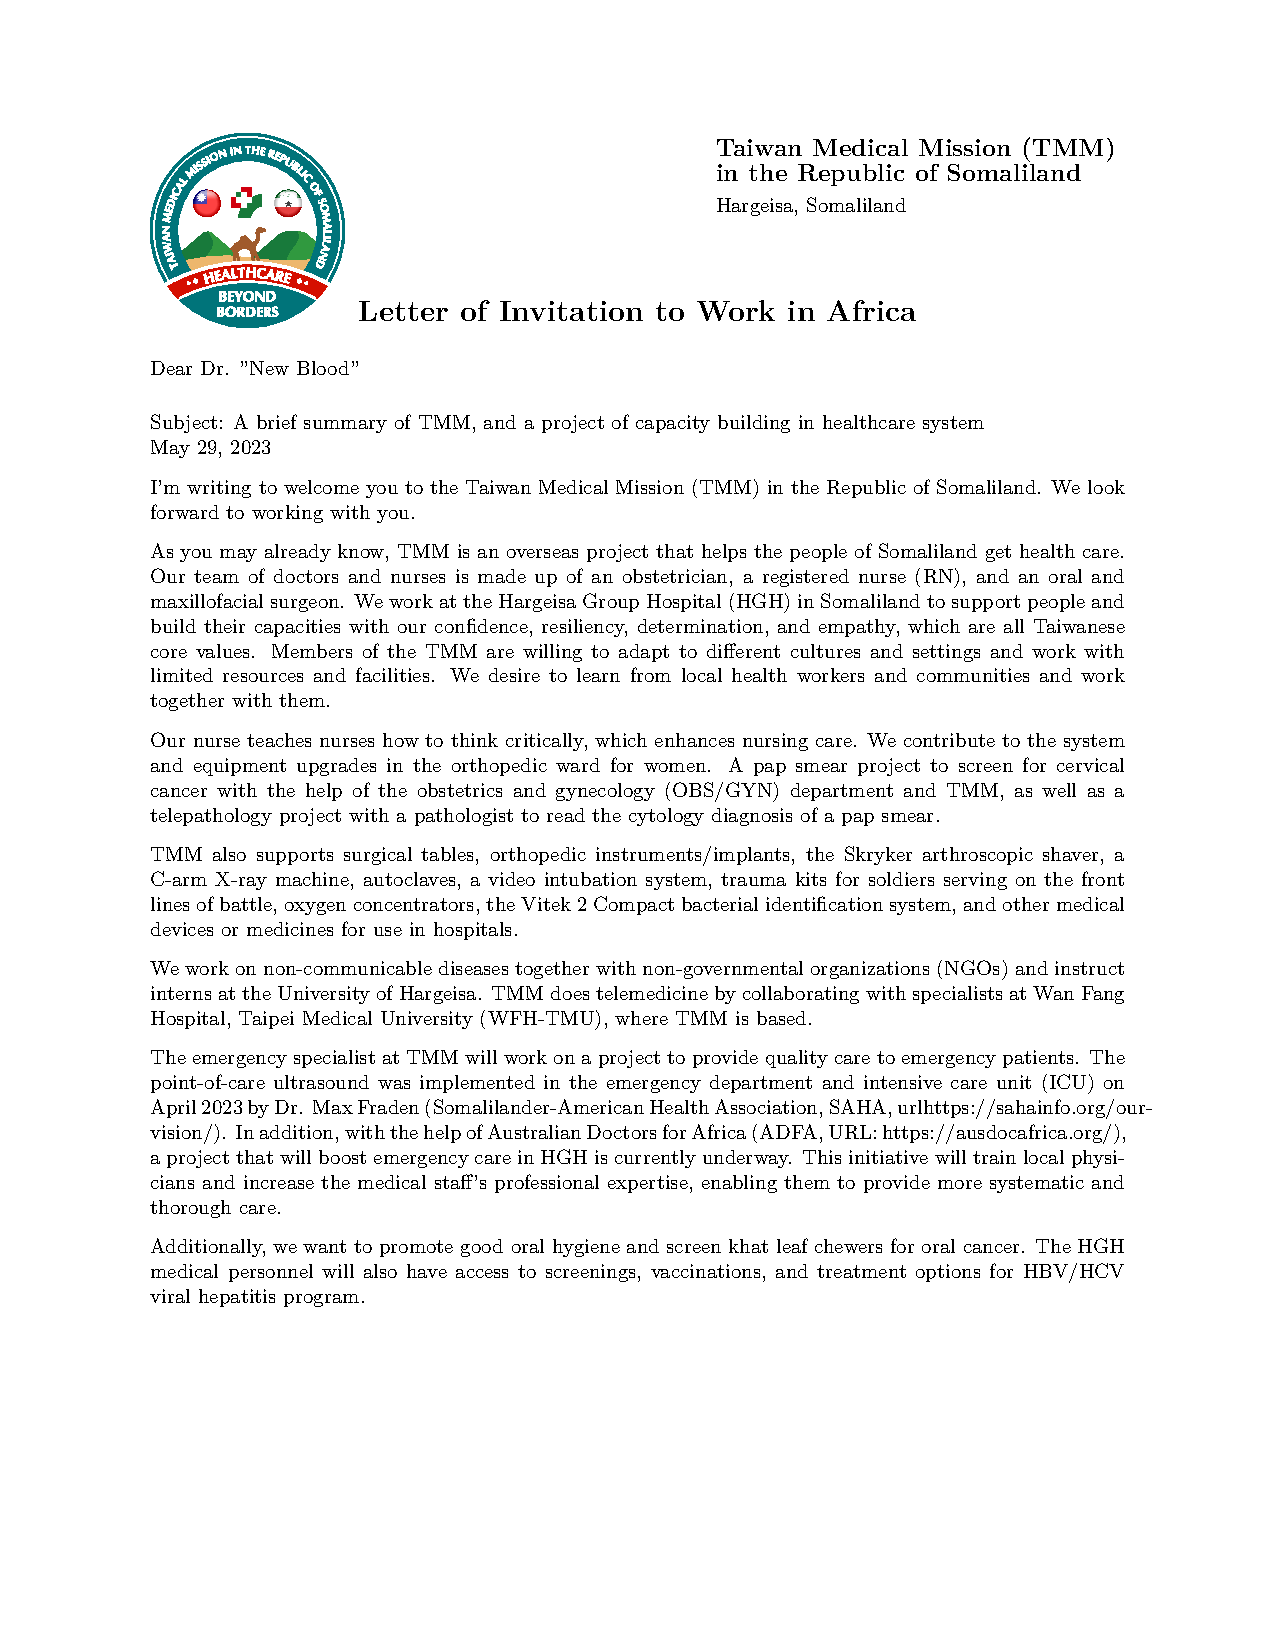
\includepdf[pages={1,2}]{ASU_WelcomeRemarks_Letter_recruit2.pdf}

\end{document}



%%%%%%%% spared TMU hospitals %^%%%%%%%%%%%%%%%%%%%%%%%%
% Figures of TMU
\begin{minipage}{0.45\linewidth}
  \centering %456
    \begin{tikzfigure}[]
    % TMWH
    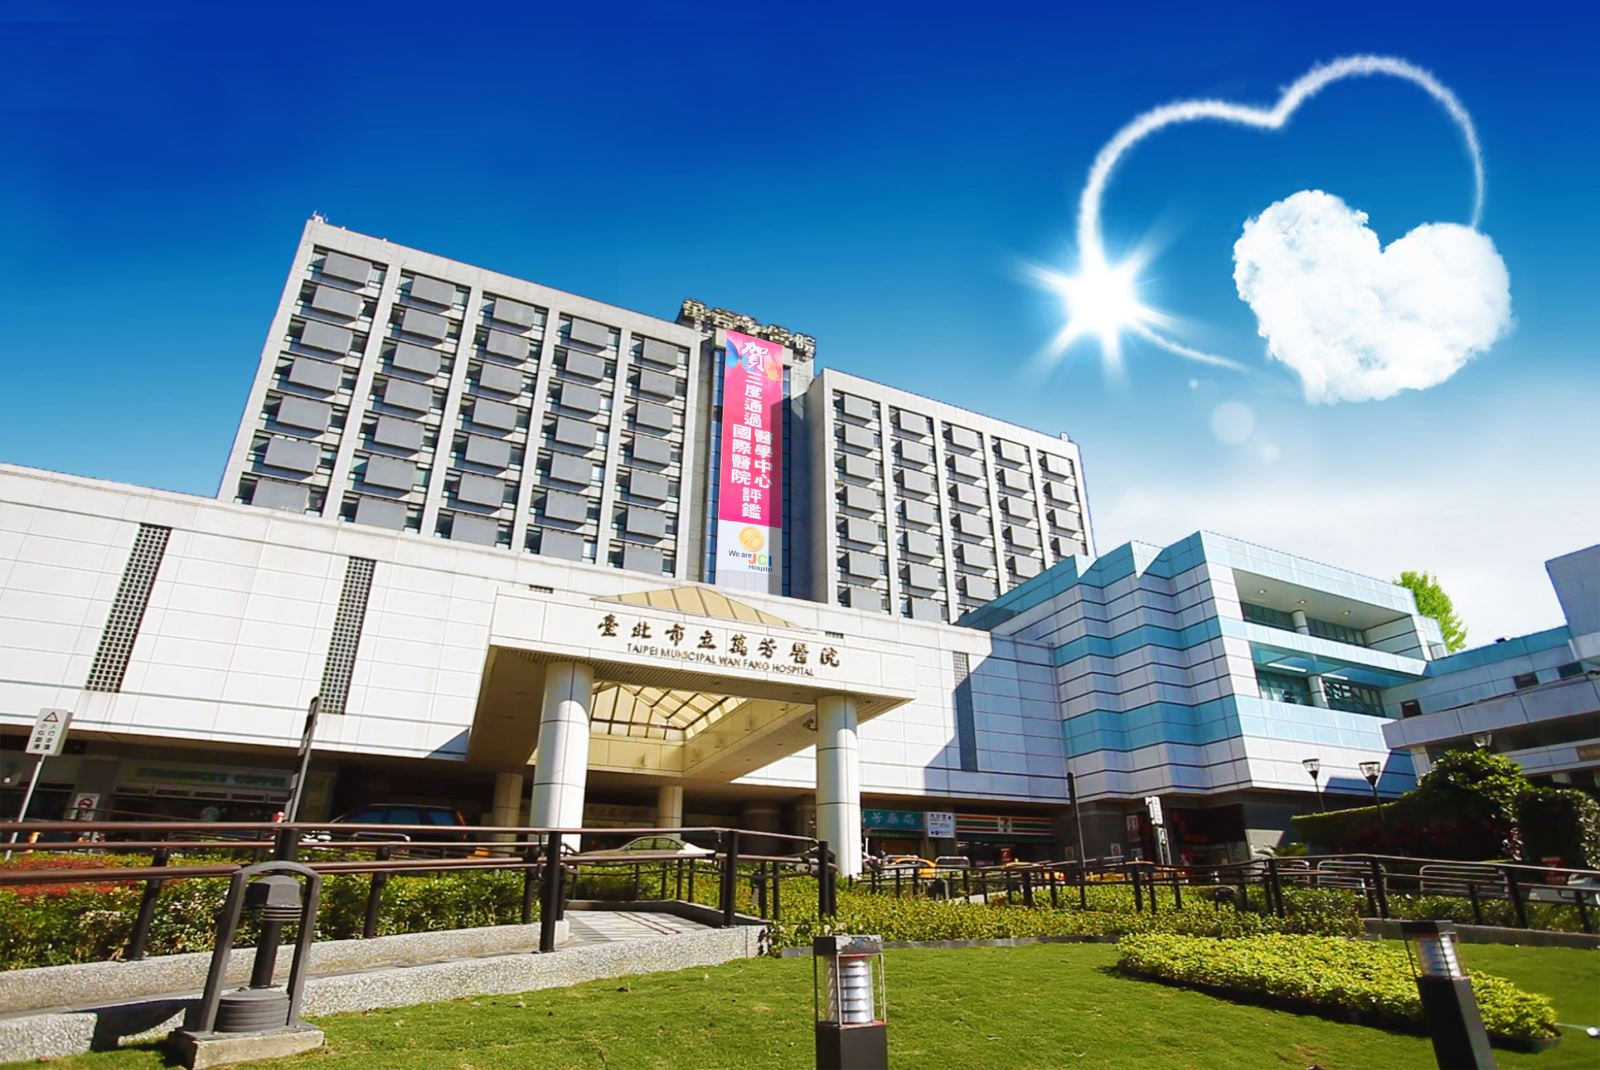
\includegraphics[width=0.7\linewidth]{5FAB9DAB-B258-4FC5-AED2-BB8F415E616F.jpeg}
    % TMUH
    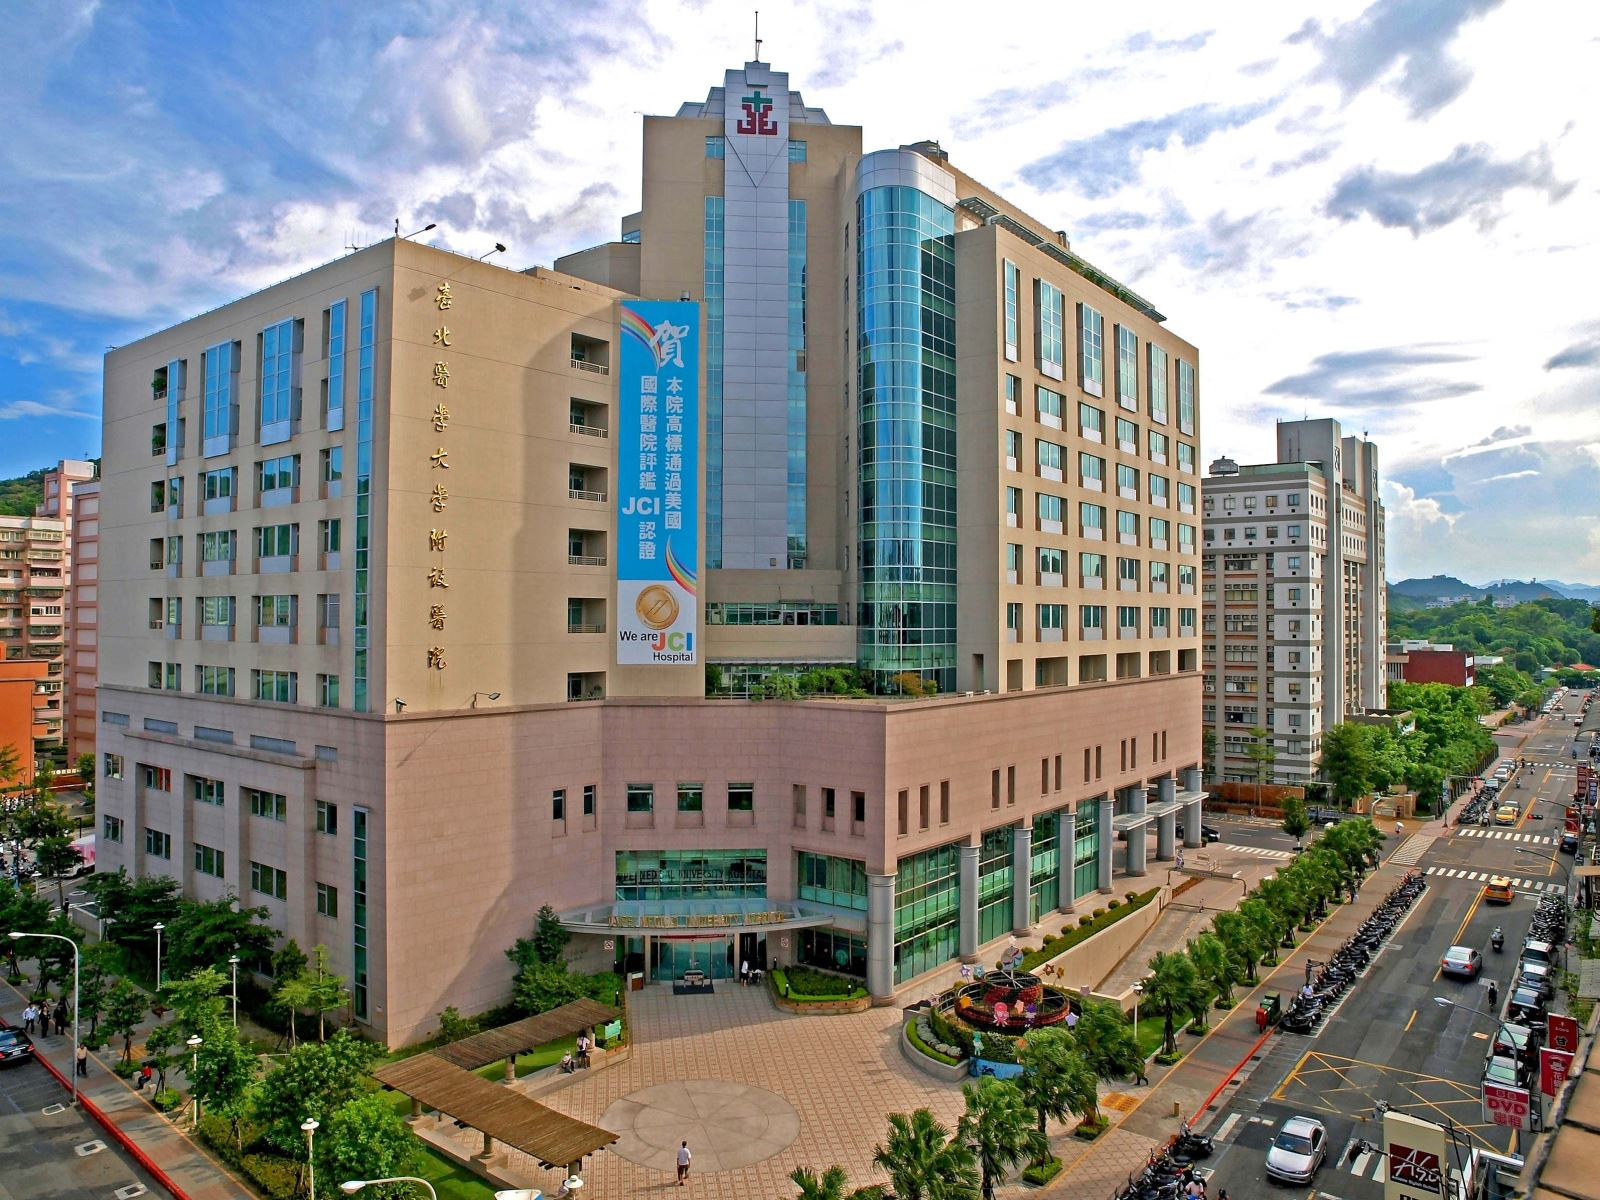
\includegraphics[width=0.7\linewidth]{5782F8B7-D58E-4601-A26D-18DFB462B6B8.jpeg}
    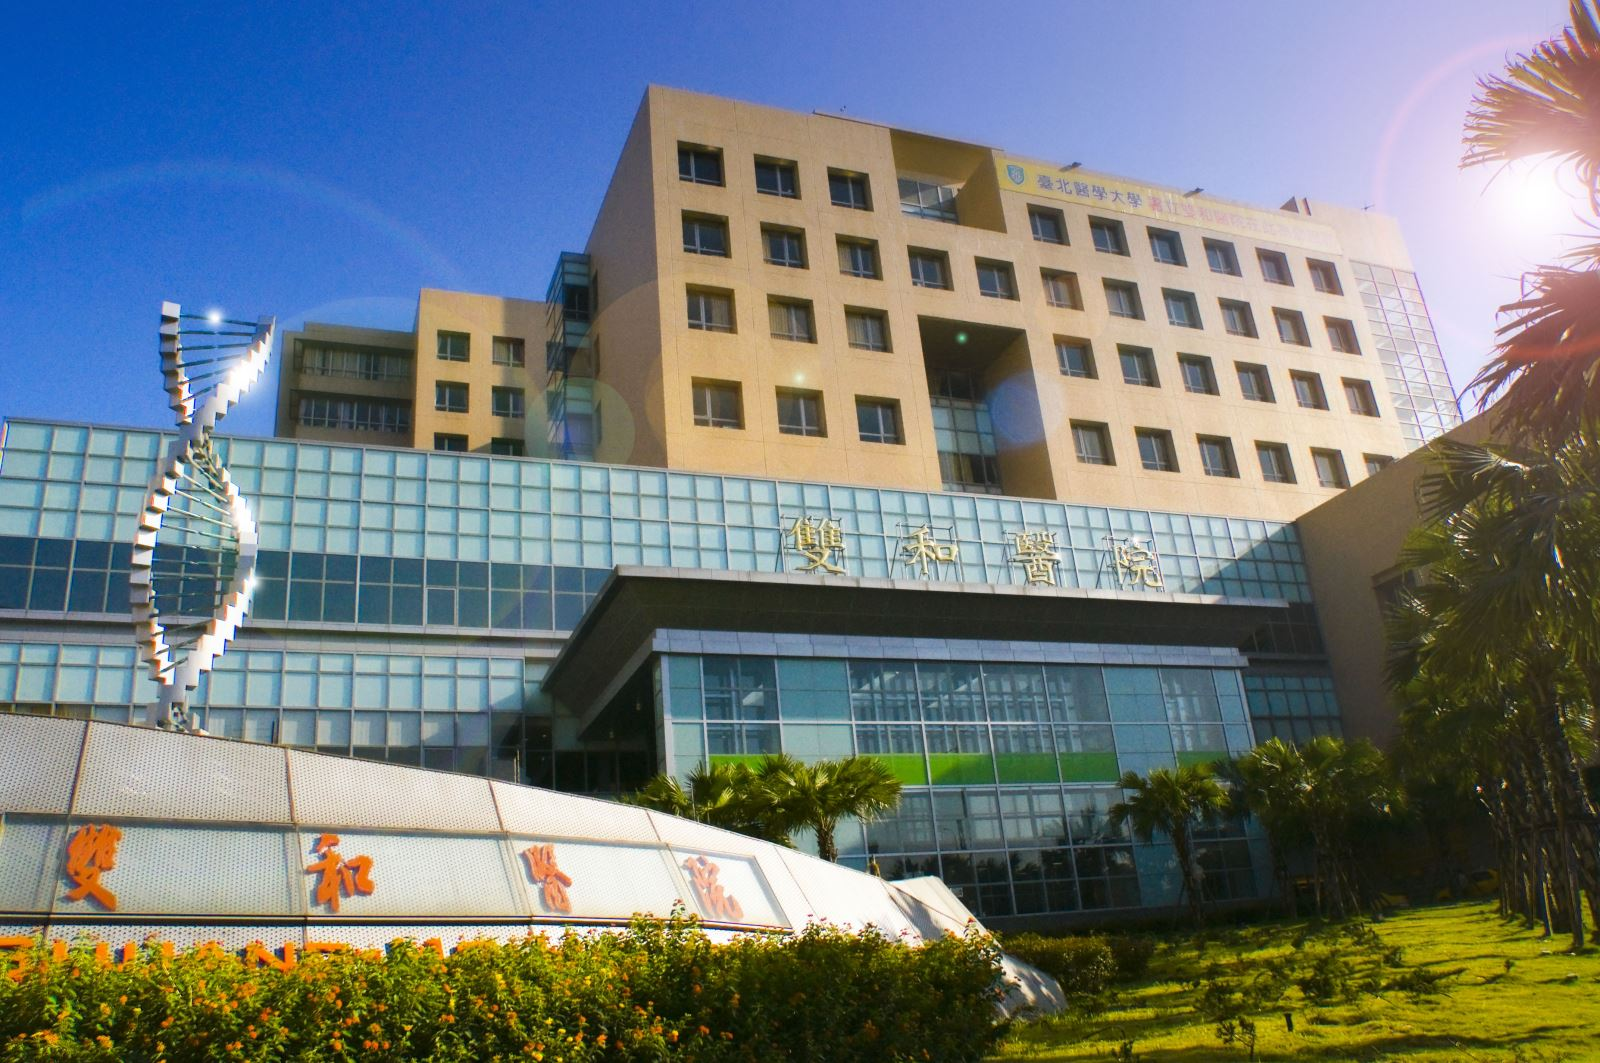
\includegraphics[width=0.7\linewidth]{10885B17-3876-4B24-B689-4B1ACDB21AB3.jpeg}
    \end{tikzfigure}
\end{minipage}\hfill
\begin{minipage}{0.45\linewidth}
  \centering
%\innerblock{TMU's Hospitals}{
    \begin{tikzfigure}[]
    %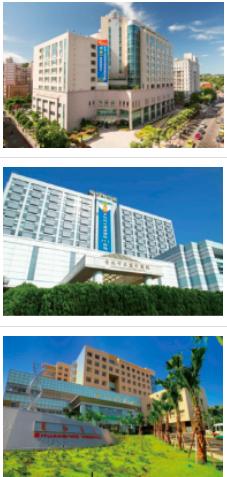
\includegraphics[width=0.5\linewidth]{TMU123.jpg}
    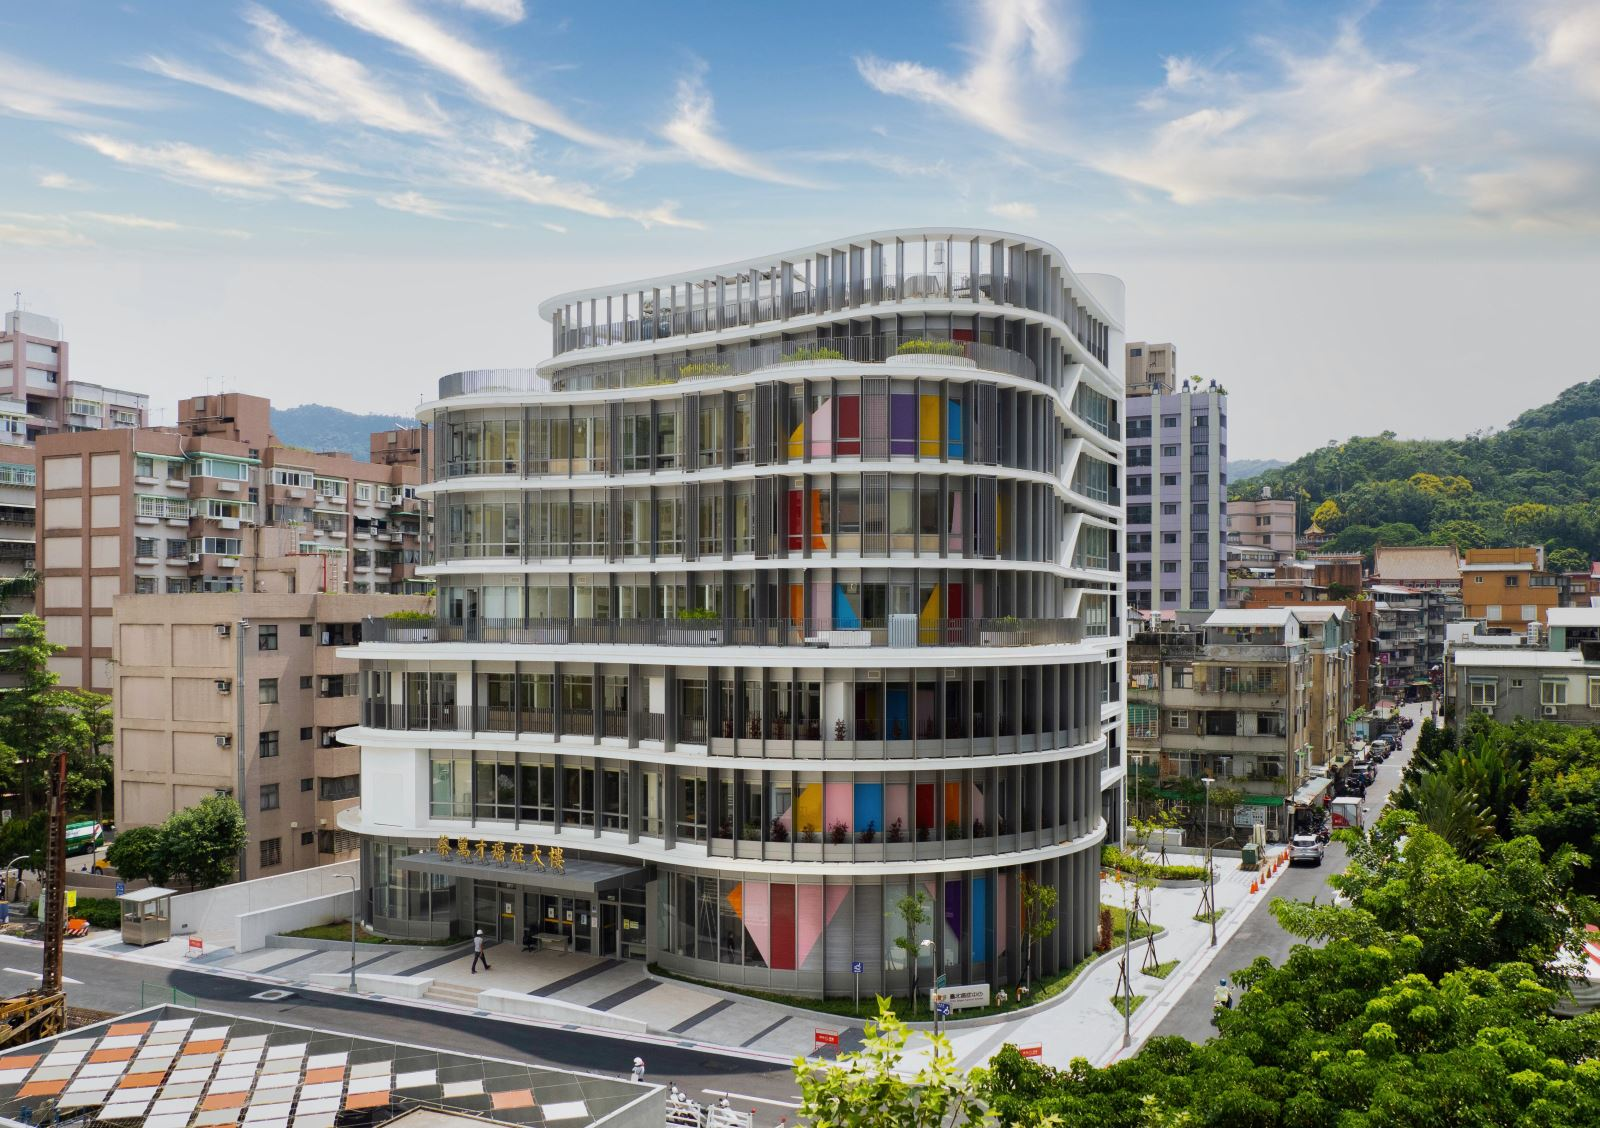
\includegraphics[width=0.75\linewidth]{295B6224-4030-47C6-9742-E3874C20445E.jpeg}
    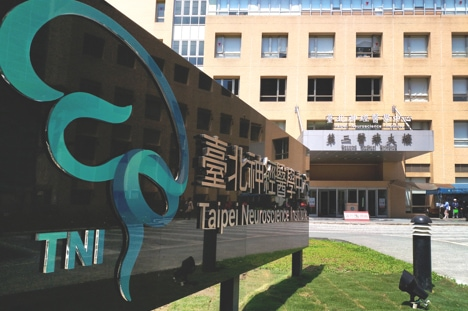
\includegraphics[width=0.75\linewidth]{6C597AEE-0ADA-4AC1-BA50-C500B9B911E0.jpeg}
    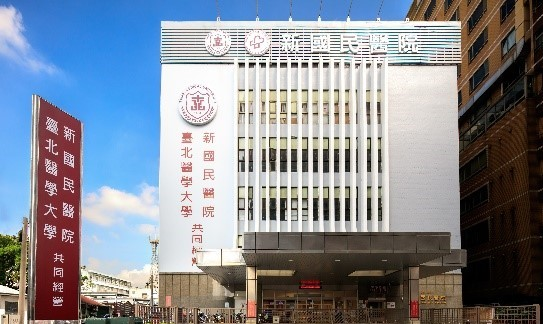
\includegraphics[width=0.75\linewidth]{17E0CB16-55CA-4F23-9A3A-F70CAE5FE133.jpeg}
\end{tikzfigure}
\end{minipage}


%%%

\block{Welcome to Taipei}{%
\begin{minipage}{0.3\linewidth}
  \centering
    \begin{tikzfigure}[Biomedical research]
    
\includegraphics[width=0.6\linewidth]{qrcode.jpeg}
    %TMU_QR_sholar.png}
%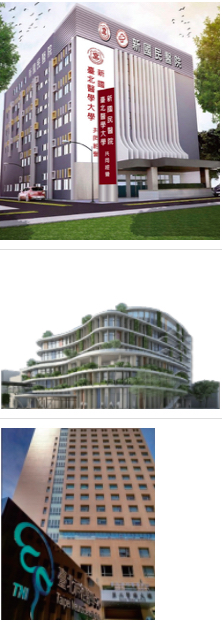
\includegraphics[width=0.5\linewidth]{TMU456.jpg}
    \end{tikzfigure}
\end{minipage}\hfill
\begin{minipage}{0.3\linewidth}
  \centering
\begin{tikzfigure}[Endoscopic simulation]
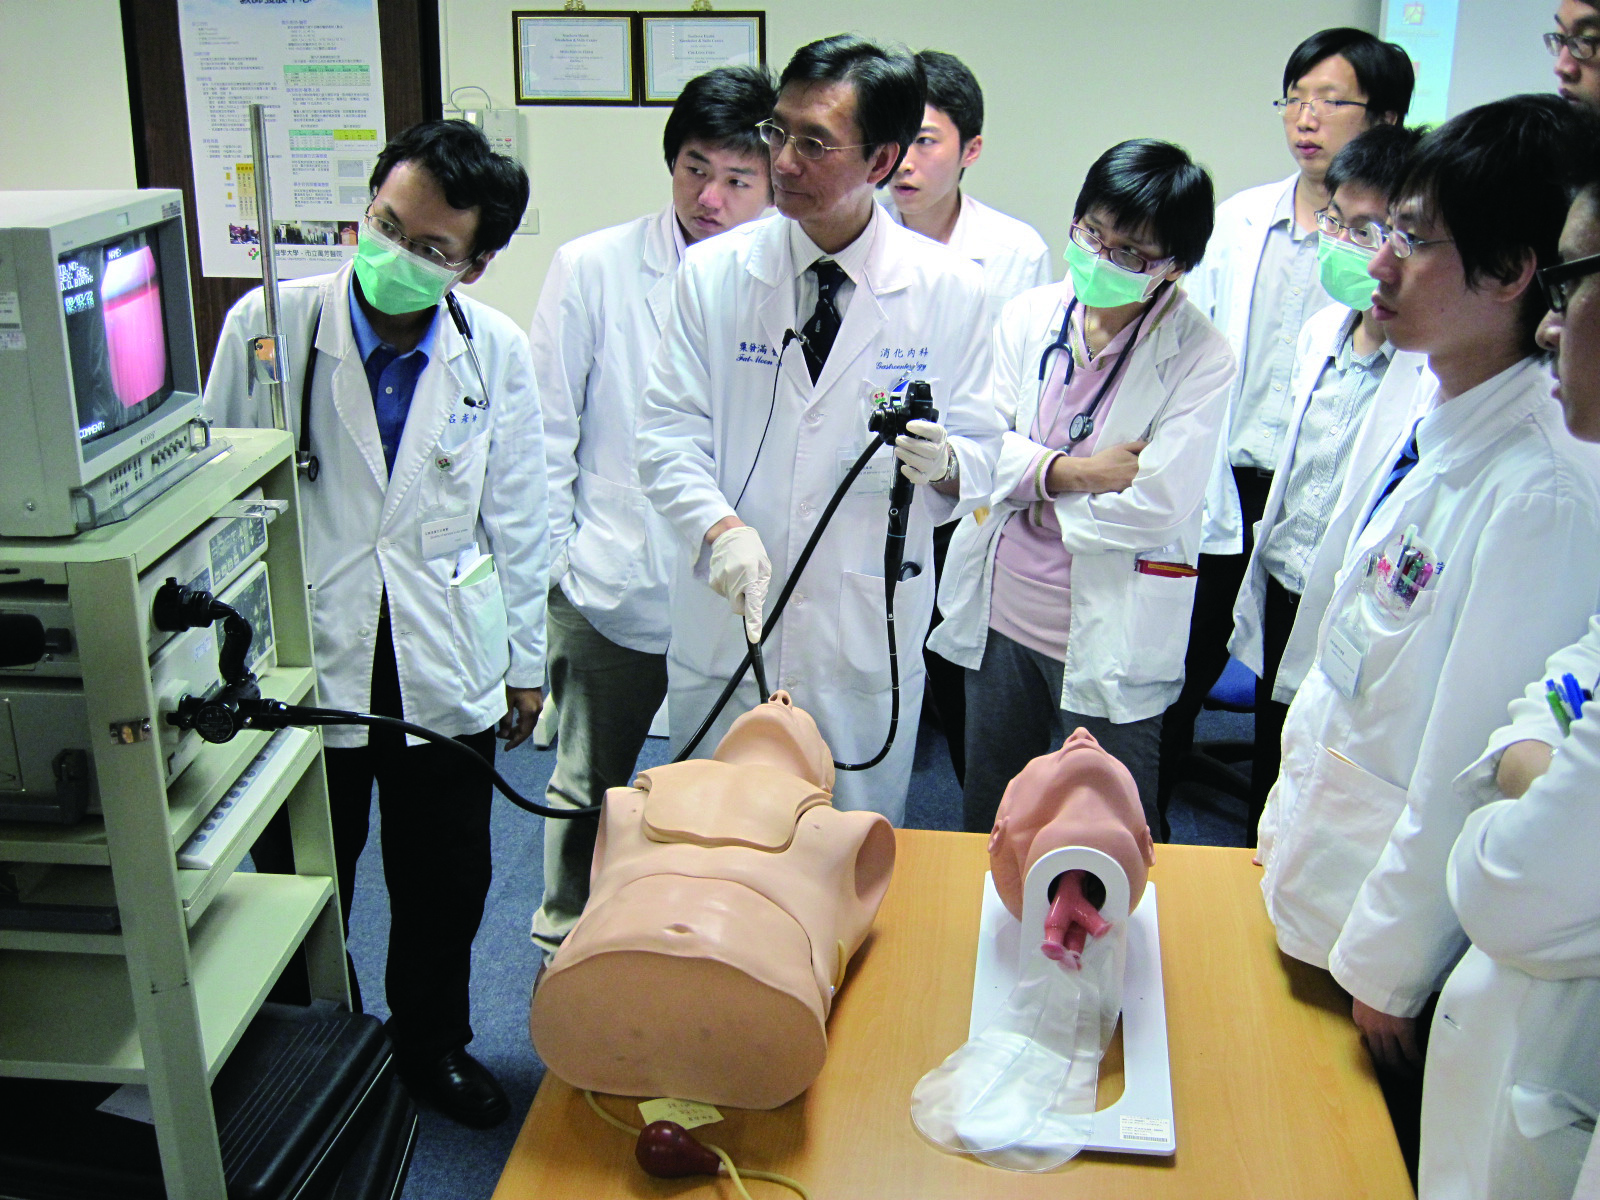
\includegraphics[width=0.7\linewidth]{2萬芳醫院中英文簡介照片.jpg}
\end{tikzfigure}  
\end{minipage}\hfill
\begin{minipage}{0.3\linewidth}
  \centering
\begin{tikzfigure}[Medical travel]

\includegraphics[width=0.65\linewidth]{qrcode.66164813.jpg}
\end{tikzfigure}
\end{minipage}

%(* photos courtesy of Studyportals B.V., and Public Relation \& Publishing Section, TMU Secretariat)
} % end of block


%%%

\column{0.6}
\block{Time Activity}{
11:00 Opening\\
11:05 Presentation of Handover Items\\
} % end of block

%\column{0.5}
%\innerblock{}{
%Opening\\
%Presentation of Handover Items
%} % end of block

\column{0.4}
\block{Speaker}{
Dr. Hassan Mohamoud Nour (Master of Ceremony)\\
Dr. Tex LH Chi (Chief of TMM)\\
} % end of block
